\section{Transformation of Variables}

This section groups the technical tools that underpin sampling distributions. The distributions studied here (Z, t, $\chi^2$, F) are the backbone of classical statistical inference and appear recurrently in data science problems.


A frequent question in statistics is: if $X$ has a known distribution and we define $Y = g(X)$ for some function $g$, what is the distribution of $Y$?

\subsection{Linear Transformation}

\begin{teorema}[Affine Transformation]
If $X$ is a random variable with mean $\mu_X$ and variance $\sigma_X^2$, and $Y = aX + b$ with $a \neq 0$, then
\begin{align}
 \label{eq:3.2.1}
 \mu_Y &= a\mu_X + b, \\
 \label{eq:3.2.2}
 \sigma_Y^2 &= a^2\sigma_X^2.
\end{align}
Furthermore, if $X$ has cumulative distribution function $F_X$, then
$F_Y(y) = F_X\!\left(\frac{y-b}{a}\right)$.
\end{teorema}

\begin{ejemplo}
 \label{exmp:3.2.1}
If $X \sim N(\mu, \sigma^2)$ and $Y = aX + b$ with $a \neq 0$, then
$Y \sim N(a\mu + b, a^2\sigma^2)$. This is the \emph{reproductive property} of the normal distribution under linear transformations.
\end{ejemplo}

\subsection{Change of Variable Theorem}

For more general transformations, we need the following result.

\begin{teorema}[Change of Variable, Monotone Case]
Let $X$ be a continuous random variable with density $f_X$, and $g$ a strictly monotone and differentiable function. If $Y = g(X)$ and $g^{-1}$ denotes the inverse of $g$, then the density of $Y$ is
\begin{align}
 \label{eq:3.2.3}
 f_Y(y) = f_X\!\left(g^{-1}(y)\right) \cdot \left|\frac{d}{dy}\,g^{-1}(y)\right|,
\end{align}
for all $y$ in the range of $g$.
\end{teorema}

\begin{proof}
Suppose $g$ is increasing. For $y$ in the range of $g$,
\begin{align}
 F_Y(y) = P(Y \leq y) = P(g(X) \leq y) = P(X \leq g^{-1}(y)) = F_X(g^{-1}(y)).
\end{align}
Differentiating and applying the chain rule,
\begin{align}
 f_Y(y) = \frac{d}{dy} F_X(g^{-1}(y)) = f_X(g^{-1}(y)) \cdot \frac{d}{dy} g^{-1}(y).
\end{align}
The decreasing case is analogous, taking the absolute value.
\end{proof}

\begin{observacion}[Alternative Form]
If we write $x = g^{-1}(y)$ and denote $J(y) = \frac{dx}{dy}$ the Jacobian of the inverse transformation, the formula can be rewritten as
\begin{align}
 \label{eq:3.2.4}
 f_Y(y) = f_X(x)\,|J(y)|, \quad \text{where } x = g^{-1}(y).
\end{align}
In higher dimensions, $|J(y)|$ is the absolute value of the Jacobian determinant.
\end{observacion}

\begin{ejemplo}
 \label{exmp:3.2.2}
Let $X \sim \text{Exp}(1)$ with density $f_X(x) = e^{-x}$ for $x > 0$. Find the distribution of $Y = e^X$.
\end{ejemplo}

\begin{solucion}
The transformation $g(x) = e^x$ is strictly increasing from $(0, \infty)$ to $(1, \infty)$, with inverse $g^{-1}(y) = \ln y$. Furthermore, $\frac{d}{dy}\ln y = 1/y$.

By the change of variable theorem, for $y > 1$:
\begin{align}
 f_Y(y) = f_X(\ln y) \cdot \frac{1}{y} = e^{-\ln y} \cdot \frac{1}{y} = \frac{1}{y} \cdot \frac{1}{y} = \frac{1}{y^2}.
\end{align}

Therefore, $Y$ has density $f_Y(y) = 1/y^2$ for $y > 1$ (a Pareto distribution with parameter $\alpha = 1$).
\end{solucion}

\begin{ejemplo}
 \label{exmp:3.2.3}
Let $X \sim N(\mu, \sigma^2)$. Find the distribution of $Y = e^X$ (the \emph{log-normal} distribution).
\end{ejemplo}

\begin{solucion}
The transformation $g(x) = e^x$ is increasing, with inverse $g^{-1}(y) = \ln y$. The density of $X$ is
\begin{align}
 f_X(x) = \frac{1}{\sigma\sqrt{2\pi}}\,\exp\!\left(-\frac{(x-\mu)^2}{2\sigma^2}\right).
\end{align}

Applying the theorem, for $y > 0$:
\begin{align}
 f_Y(y) &= f_X(\ln y) \cdot \frac{1}{y} \\
 &= \frac{1}{\sigma\sqrt{2\pi}}\,\exp\!\left(-\frac{(\ln y - \mu)^2}{2\sigma^2}\right) \cdot \frac{1}{y}.
\end{align}

Therefore, $Y$ follows a log-normal distribution $LN(\mu, \sigma^2)$.
\end{solucion}

\begin{ejemplo}
 \label{exmp:3.2.4}
Let $X \sim U(0, 2\pi)$ be uniformly distributed. Find the distribution of $Y = \sin(X)$ (non-monotone case).
\end{ejemplo}

\begin{solucion}
The function $g(x) = \sin x$ is not monotone on $(0, 2\pi)$: it reaches a maximum of $1$ at $x = \pi/2$ and a minimum of $-1$ at $x = 3\pi/2$. Each value $y \in (-1, 1)$ has two preimages: $x_1 = \arcsin y$ and $x_2 = \pi - \arcsin y$.

Using the formula for the non-monotone case,
\begin{align}
 f_Y(y) &= \sum_{x: \sin x = y} f_X(x) \cdot \left|\frac{dx}{dy}\right| \\
 &= \frac{1}{2\pi}\cdot\frac{1}{\sqrt{1-y^2}} + \frac{1}{2\pi}\cdot\frac{1}{\sqrt{1-y^2}} \\
 &= \frac{1}{\pi\sqrt{1-y^2}}, \quad y \in (-1, 1).
\end{align}

This is the density of the \emph{arcsine distribution}, which appears in the \emph{random walk}.
\end{solucion}

\subsection{Common Transformations}

\begin{observacion}
The following transformations are useful for \emph{normalizing} data or stabilizing variances:
\begin{itemize}
 \item $Y = \ln X$: compresses large values, expands values close to $0$.
 \item $Y = \sqrt{X}$: smooths out the skewness of count data.
 \item $Y = X^{1/3}$: alternative to the square root for data with pronounced skewness.
 \item \emph{Box-Cox}: $Y = (X^\lambda - 1)/\lambda$ for $\lambda \neq 0$; $Y = \ln X$ for $\lambda = 0$. Optimizes normality.
\end{itemize}
\end{observacion}

\lstinputlisting[language=Python]{../code/distribuciones-muestreo/transformacionesVariables.py}

\begin{figure}
 \centering
 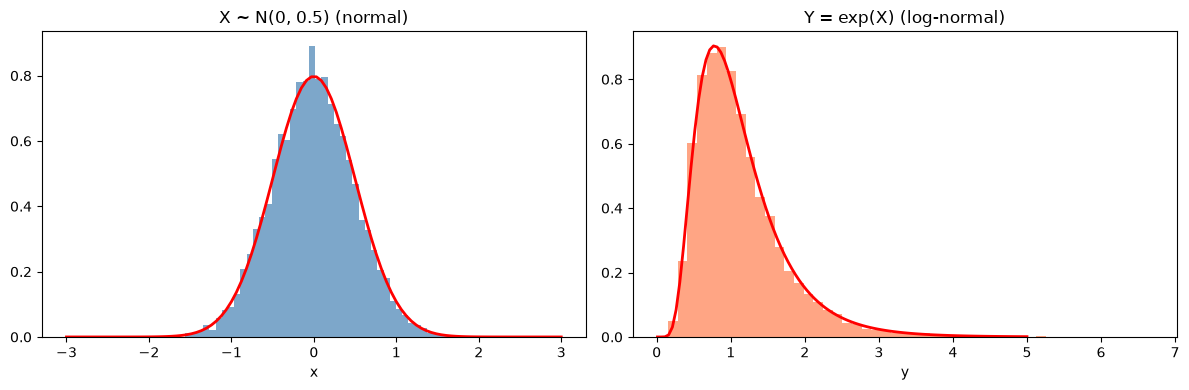
\includegraphics[height=7cm,keepaspectratio=true]{./pe/transformaciones.png}
 % transformaciones.png: 0x0 pixel, 300dpi, 0.00x0.00 cm, bb=
 \caption{Exponential transformation: from normal to log-normal.}
 \label{fig:3.2.1}
\end{figure}
